\hypertarget{Checkpoint_8cpp}{}\section{src/\+Checkpoint.cpp File Reference}
\label{Checkpoint_8cpp}\index{src/\+Checkpoint.\+cpp@{src/\+Checkpoint.\+cpp}}


Contains definitions for the Checkpoints class.  


{\ttfamily \#include \char`\"{}../headers/\+Checkpoint.\+h\char`\"{}}\\*
Include dependency graph for Checkpoint.\+cpp\+:\nopagebreak
\begin{figure}[H]
\begin{center}
\leavevmode
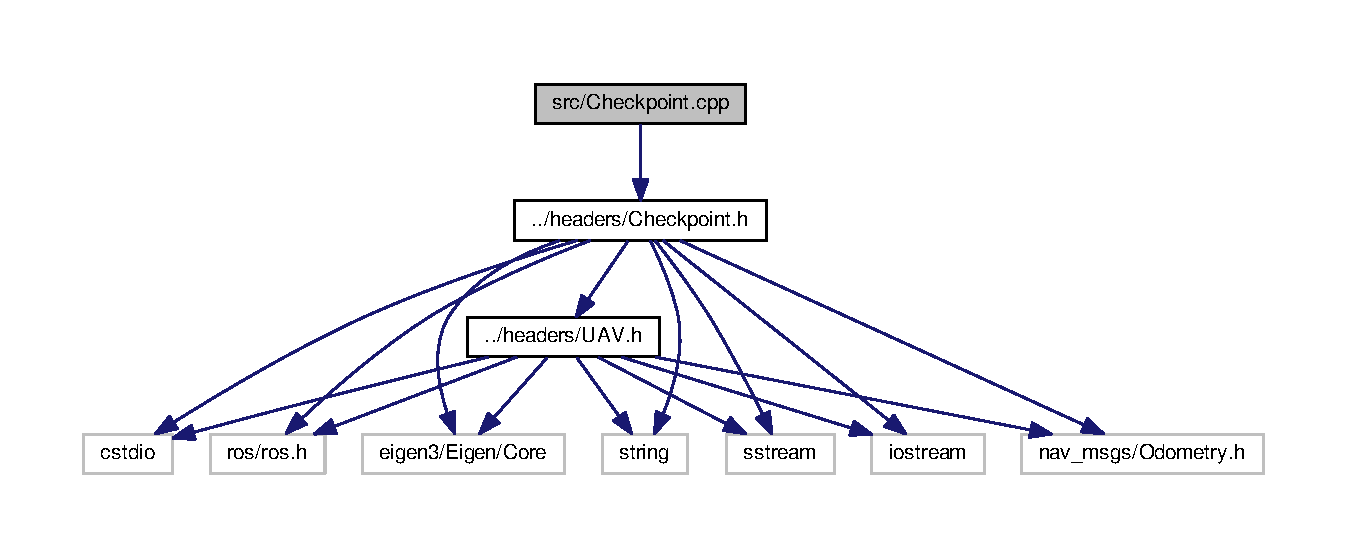
\includegraphics[width=350pt]{Checkpoint_8cpp__incl}
\end{center}
\end{figure}


\subsection{Detailed Description}
Contains definitions for the Checkpoints class. 

Contains function definitions for the \hyperlink{classCheckpoint}{Checkpoint} class. The \hyperlink{classCheckpoint}{Checkpoint} class consists of functions required for detecting that the \hyperlink{classUAV}{U\+AV} swarm has flown through a particular location and for measuring time of flight. 